\subsection{Penalização por proximidade}
% TODO

\begin{figure}[H]
  \centering
  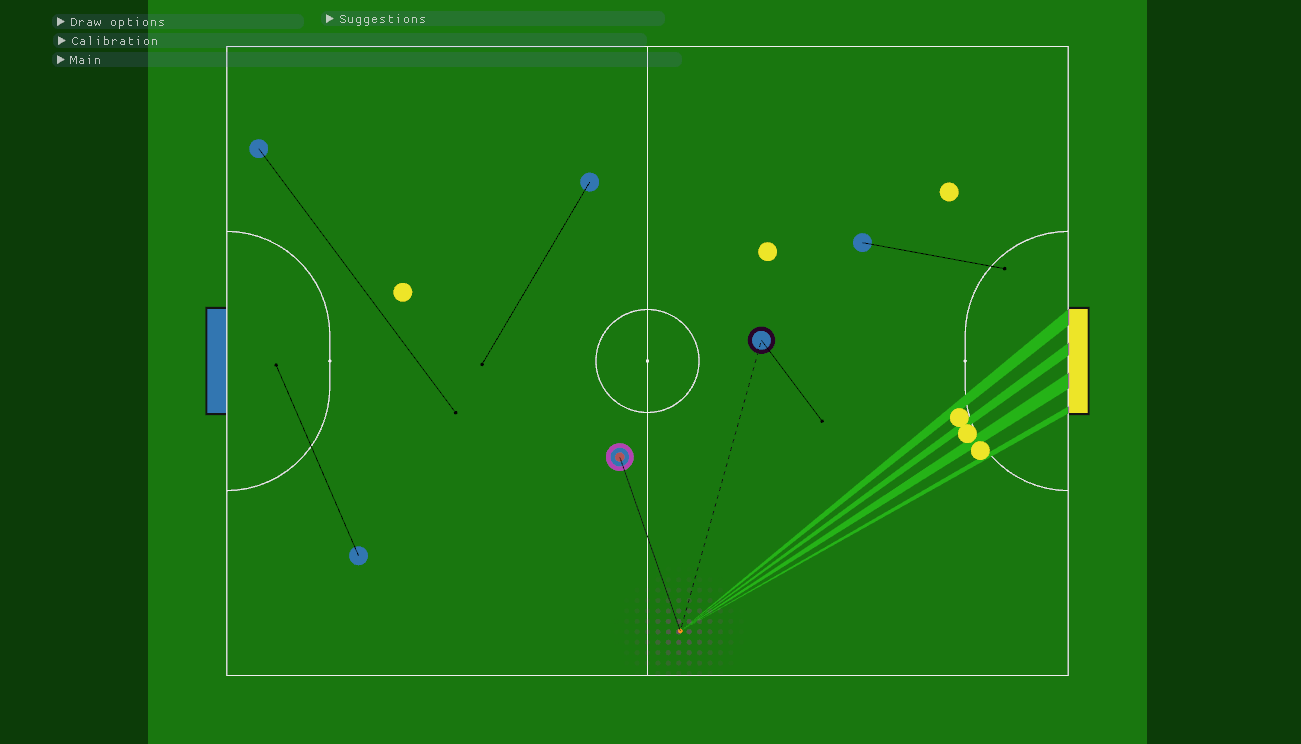
\includegraphics[width= 0.8\linewidth]{result/default_atq}
  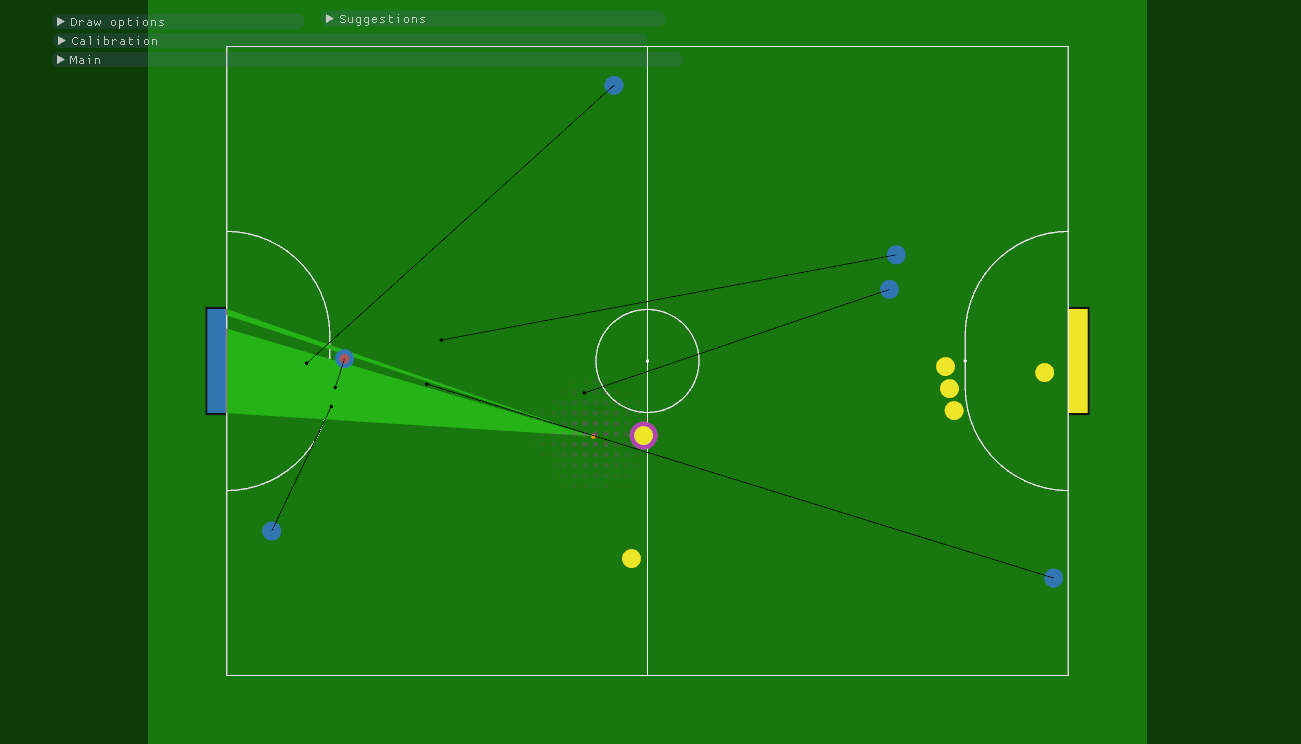
\includegraphics[width= 0.8\linewidth]{result/default_def}
  \caption{Planejamento com os parâmetros iniciais no
           ataque (acima) e na defesa (abaixo)}\label{fig:default}
\end{figure}
